\documentclass{article}
\usepackage{amsmath}
\usepackage{amssymb}
\usepackage{algorithm}
\usepackage{float}
\usepackage{color}
\usepackage{multicol}
\usepackage{forloop}
\usepackage{graphicx}
\usepackage[margin=0.8in]{geometry}
\usepackage{caption}
\usepackage{enumerate}
\graphicspath{ {.} }
\title{STAT 2509B4 \\
	\large{Assignment 3}}
\author{Krystian Wojcicki, 101001444}
\date{Winter 2020}

\begin{document}
\maketitle

\begin{enumerate}[1.]

\item
\textbf{Indicate whether or not each of the following models can be treated as an multiple linear
regression (MLR) model:}
\begin{enumerate}[(i)]
\item  $y = \beta_0 + \beta_1x_1 + \beta_2x_2 + \beta_3x_1x_2 + \epsilon $, can be treated as MLR
\item  $y = (e^{\beta_0 + \beta_1x_1 + \beta_2x_2^2})\epsilon$, cannot be treated as MLR
\item  $y = \beta_0 + \beta_1x_1 + \beta_2e^{x_1} + \epsilon$, can be treated as MLR
\item  $y = \beta_0 + \beta_1x_1 + \beta_2x_1^2 + \beta_3x_1^3 + \beta_4x_2 + \epsilon$, can be treated as MLR
\item $y = \beta_0e^{\beta_1x_1 + \beta_2x_2} + \epsilon$, cannot be treated as MLR
\end{enumerate}

\item
\textbf{ A medical study was conducted to study the relationship between infants’ systolic blood
pressure and two explanatory variables, age (days) and weight (kg). The data for 25 infants
are given below..:\\
\begin{center}
 \begin{tabular}{||c c c||} 
 \hline
Age ($x_1)$ & Weight ($x_2$) & Systoli BP (y) \\ [0.5ex] 
 \hline\hline
3 & 2.61 & 80 \\
\hline
4 & 2.67 & 90 \\
\hline
5 & 2.98 & 96\\
\hline
6 & 3.98 & 102\\
\hline
3 & 2.87 & 81\\
\hline
4 & 3.41 & 96\\
\hline
5 & 3.49 & 99\\
\hline
6 & 4.03 & 110\\
\hline
3 & 3.41 & 88\\
\hline
4 & 2.81 & 90\\
\hline
5 & 3.24 & 100\\
\hline
6 & 3.75 & 102\\
\hline
3 & 3.18 & 86\\
\hline
4 & 3.13 & 93\\
\hline
5 & 3.98 & 101\\
\hline
6 & 4.55 & 103\\
\hline
3 & 3.41 & 86\\
\hline
4 & 3.35 & 91\\
\hline
5 & 3.75 & 100\\
\hline
6 & 3.83 & 105\\
\hline
3 & 3.18 & 84\\
\hline
4 & 3.52 & 91\\
\hline
5 & 3.49 & 95\\
\hline
6 & 3.81 & 104\\
\hline
6 & 4.03 & 107  \\ [1ex]
 \hline
\end{tabular}
\end{center}
}
\begin{enumerate}[(a)]
\item \textbf{State all the assumptions that are necessary for the statistical inference under the MLR model.: } \\
Model $y = \beta_0 + \beta_1x_1 + \beta_2x_2 + \epsilon, n = 25$ \\
Assumptions
  \begin{enumerate}[(1)]
   \item $X_1, X_2$ are observed without error
   \item $\epsilon$'s are independently distributed
   \item $\epsilon$'s have common mean 0 in other words $E(\epsilon) = 0$ for all $X_1,X_2$.
   \item $\epsilon$'s have common/constant variance $\sigma^2$ meaning $Var(\epsilon) = \sigma^2$ for all $X_1,X_2$
  \item $\epsilon \sim N(0, \sigma^2)$ for any value of $X_1, X_2$
\end{enumerate}

\item \textbf{Use matrices to compute the least-squares estimates of the population parameters $\beta_0$, $\beta_1$ and $\beta_2$, and obtain the fitted least-squares regression line:  \\
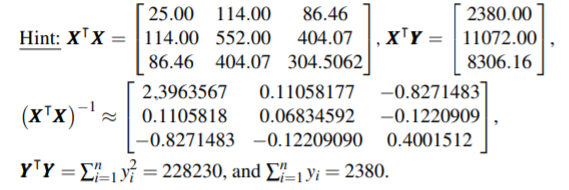
\includegraphics{a3_hint}} \\

$(X^TX)^{-1} X^TY = \begin{bmatrix}
2.3963567 & 0.11058177 & -0.8271483 \\
0.1105818 & 0.06834592 & -0.1220909 \\
-0.8271483 & -0.12209090 & 0.4001512 \\
\end{bmatrix} * 
\begin{bmatrix}
2380.00 \\
11072.00 \\
8306.16 \\
\end{bmatrix}= 
\begin{bmatrix}
57.2642 \\
5.80416 \\
3.31649 \\
\end{bmatrix} = 
\begin{bmatrix}
    \hat{\beta_0} \\
    \hat{\beta_1} \\
    \hat{\beta_2}
\end{bmatrix} = \hat{\beta}$

Therefore the fitted least squares regression line is $\hat{y} = 57.2642 + 5.80416x_1 + 3.31649x_2$

\item \textbf{ Set up the ANOVA table and test for significance of the model at the significance level of $\alpha$ = 0.05 } \\
$TSS = Y^TY - \frac{(\sum_{i=1}^{n}{y_i})^2}{n} = \sum_{i=1}^{n}{y_i^2} - \frac{(\sum_{i=1}^{n}{y_i})^2}{n}  = 228230 - \frac{2380^2}{25} = 1654$

$SSR = \hat{\beta^T}(X^TY)  - \frac{(\sum_{i=1}^{n}{y_i})^2}{n}  = \begin{bmatrix}
57.2642 & 5.80416 & 3.31649
\end{bmatrix} * \begin{bmatrix}
2380.00 \\
11072.00 \\
8306.16 \\
\end{bmatrix} - \frac{2380^2}{25} = 1523.752098$

$SSE = TSS - SSR = 1654 - 1523.752098 = 130.247902$ \\
$MSR = \frac{SSR}{k} = \frac{1523.752098}{2} = 761.876$ \\
$MSE = \frac{SSE}{n-(k+1)} = \frac{130.247902}{22} = 5.920359$ \\
$F = \frac{MSR}{MSE} = \frac{761.876}{5.920359} =128.687$ \\

\begin{center}
 \begin{tabular}{||c c c c c||} 
 \hline
Source & d.f & SS & MS & F \\ [0.5ex] 
 \hline\hline
Regression & 2 & 1523.752098 & 761.876 & 128.687 \\
 \hline
Error & 22 & 130.247902 &  5.920359 &  \\
 \hline
Total & 24  & 1654 & & \\ [1ex]
 \hline
\end{tabular}
\end{center}

$H_0: \beta_1 = \beta_2 = 0$ \\
$H_a: \text{at least one of the } \beta's \neq 0$ \\
$\alpha = 0.05$

test-statistics: $F = \frac{MSR}{MSE} = 128.687$

Rejection region, we reject $H_0$ if $F > F_{(k, n-(k+1)), \alpha} = F_{2, 22; 0.05} = 3.4434$

Since $F = 128.687 > 3.4434$, we reject $H_0$ and conclude that at a 5\% level of significance there is evidence to say there is a linear relationship between age, weight and the systolic BP.

\item \textbf{ Test whether age (x1) contributes to explaining (or predicting) the systolic blood pressure (y) under the MLR model. Use t-test with $\alpha = 0.05$. } \\

$H_0: \beta_1 = 0$ \\
$H_a: \beta_1 \neq 0$ \\
$\alpha = \to \alpha/2 =  0.025$

test statistics: $t = \frac{\hat{\beta_1}}{\sqrt{v_{11}MSE}} = \frac{5.80416}{\sqrt{0.0683459 * 5.920359}} = 9.1245$

Rejection region, we reject $H_0$ if $|t| > t_{n-(k+1), \alpha/2} = t_{22, 0.025} =  2.07383$.

Since $t =  9.1245 > 2.07$, we reject $H_0$ and conclude that at a 5\% level of significance there is evidence to say that the $x_1$ term contributes to the model.

\item \textbf{ Find the values of the coefficient of determination, $r^2$, and the adjusted $r^2$. Interpret their meanings in this problem} \\

$r^2 = \frac{SSR}{TSS} = \frac{1523.752098}{1654} = 0.9213 = 92.125\%$

In other words approximately 92.13\% of the total variation in the data is explained by the regression line. The rest is due to error.

$r_{adj}^2 = 1 - \frac{SSE/n-(k+1)}{TSS/n-1} = 1 - \frac{MSE}{TSS/n-1} = 1 - \frac{5.920359}{1654/24} = 0.9141 = 91.41\%$

Since both $r^2$ and $r_{adj}^2$ are quite high (above 80\%), both have similar values around 90\%, and since the $x_1$ term does contribute to the model, we can conclude that the model is good.

\item \textbf{ Run SAS to verify your answers to the above questions. In addition, use the SAS output to answer subquestion (d) using the partial F-test with $\alpha$ = 0.05.} See attatched SAS output

$H_0: \beta_1 = 0$ \\
$H_a: \beta_1 \neq 0$ \\
$\alpha = 0.05$ \\

full model: $y = \beta_0 + \beta_1x_1 + \beta_2x_2 + \epsilon$ \\
reduced model: $y = \beta_0 + \beta_2x_2 + \epsilon$ \\

$SSR_f = 1521.53295$ with d.f $= 2$ \\
$SSE_f = 132.46705$ with d.f $= 22$ \\
$SSR_r = 1028.63536$ with d.f $= 1$ \\
$SSE_r = 625.36464$ with d.f $=23$ \\


test statistics:
$F_{part} = \frac{ [SSR_f - SSR_r] / [df_{SSR_f} - df_{SSR_r} ] }{ SSE_f / df_{SSE_f} } = \frac{ (1521.53295 - 1028.63536) / (2 - 1) }{  132.46705 / 22} = 81.85996$

Rejection Region, we reject $H_0$ if $F_{part} > F_{(1, 22); 0.05} = 4.3009$

Since $F_{part} = 81.85996 > 4.3009$ we reject $H_0$ and conclude that at a 5\% level of significance there is enough evidence to say that the $X_1$ (age) term contributes to the model.

\end{enumerate}


\item
\textbf{An experimenter wished to compare the potencies of three different drug products. To do
this, 12 test tubes were inoculated with a culture of the virus under study and incubated for
2 days at 35C. Four dosage levels (0.2, 0.4, 0.8, and 1.6 mg per tube) were to be used from
each of the three drug products (A, B and C), with only one dose-drug product combination
for each of the 12 test-tube cultures. The data are shown in the following table \\
\begin{center}
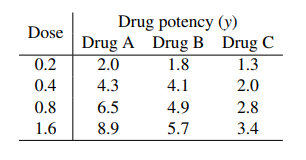
\includegraphics{a3_q3}
\end{center}
Let\\
}
$x_1 = \ln(dose), x_2 = \begin{cases} 1, & \mbox{if drug B} \\ 0, & \mbox{otherwise} \end{cases}, x_3 = \begin{cases} 1, & \mbox{if drug C} \\ 0, & \mbox{otherwise} \end{cases}$
\textbf{
and $y = \mbox{drug potency}$. Consider the following MLR model.
$y = \beta_0 + \beta_1x_1 + \beta_2x_2 + \beta_3x_3 + \beta_4x_1x_2 + \beta_5x_1x_3 + \epsilon$.
Run SAS to test whether the 3 lines corresponding to the effects of the 3 drugs are parallel
(i.e. whether these 3 lines have the same slope). Use $\alpha$ = 0.05.
}

Full model: $y = \beta_0 + \beta_1x_1 + \beta_2x_2 + \beta_3x_3 + \beta_4x_1x_2 + \beta_5x_1x_3 + \epsilon$

If drug A: $y = \beta_0 + \beta_1x_1 + \epsilon$

If drug B: $y = \beta_0 + \beta_1x_1 + \beta_2 + \beta_4x_1 + \epsilon = (\beta_0 + \beta_2) + (\beta_1 + \beta_4)x_1 + \epsilon$

If drug C: $y = \beta_0 + \beta_1x_1 + \beta_3 + \beta_5x_1 + \epsilon = (\beta_0 + \beta_3) + (\beta_1 + \beta_5)x_1 + \epsilon$ \\

Test if any of the 3 drug lines are parallel or have the same slope: \\
$H_0: \beta_4 = \beta_5 = 0$ \\
$H_a:$ at least one of the $\beta$'s $\neq 0$. \\
$\alpha = 0.05$ \\

Reduced model $y = \beta_0 + \beta_1x_1 + \beta_2x_2 + \beta_3x_3 + \epsilon$

$SSR_f = 55.29350$ with d.f. $= 5$ \\
$SSE_f = 0.68900$ with d.f. $=6$ \\
$SSR_r = 48.84417$ with d.f. $= 3$ \\
$SSE_r = 7.13833$ with d.f. $= 8$ \\

$F_{part} = \frac{ [SSR_f - SSR_r] / [df_{SSR_f} - df_{SSR_r} ] }{ SSE_f / df_{SSE_f} } = \frac{ (55.29350 - 48.84417)/(5 - 3) }{ 0.68900 / 6} = 28.081$

Rejection Region, we reject $H_0$ if $F_{part} > F_{(2,6); 0.05} = 5.14$.

Since $F_{part} = 28.081 > 5.14$ we reject $H_0$ and conclude that at a 5\% level of significance there is enough evidence to  say that the slopes of the 3 drug lines are not parallel.

\end{enumerate}

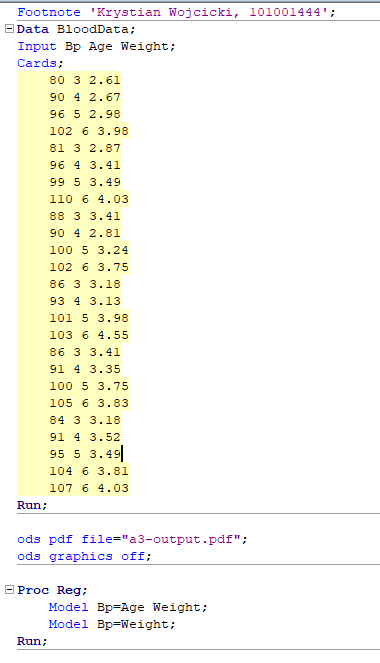
\includegraphics{a3_sascode1} \\
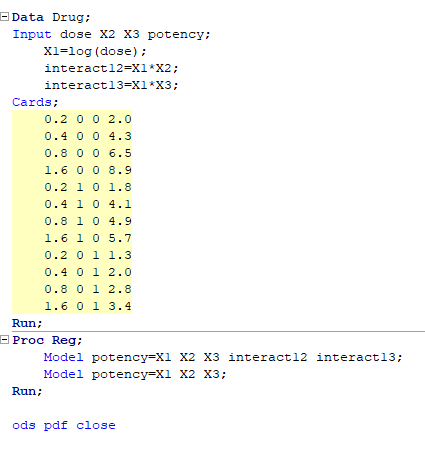
\includegraphics{a3_sascode2}

\end{document}